\renewcommand{\theequation}{\theenumi}
\begin{enumerate}[label=\thesection.\arabic*.,ref=\thesection.\theenumi]
\numberwithin{equation}{enumi}

\item Line $5x-y=5$ can be represented in vector form as,
\begin{align}
\label{eq:firstline}
\myvec{5&-1}\vec{X}=5
\end{align}

\item Line $3x-y=3$ can be represented in vector form as,
\begin{align}
\label{eq:secondline}
\myvec{3&-1}\vec{X}=3
\end{align}
%
Also the equation of y axis is 
\begin{align}
\myvec{1&0}\vec{X}=0
\label{eq:yaxis}
\end{align}

Let line \ref{eq:firstline} and  line \ref{eq:secondline} meet at point $\vec{A}$.Then, 
\begin{align}
\myvec{5&-1\\3&-1}\vec{A} =\myvec{5\\3}
\\
\vec{A}=\myvec{5\\3}{\myvec{5&-1\\3&-1}}^{-1}
\\
\vec{A}=\myvec{1\\0}
\end{align}

Let line \ref{eq:firstline} and  line \ref{eq:yaxis} meet at point $\vec{B}$. Then, 
\begin{align}
\myvec{5&-1\\1&0}\vec{B} =\myvec{5\\0}
\\
\vec{B}=\myvec{5\\0}{\myvec{5&-1\\1&0}}^{-1}
\\
\vec{B}=\myvec{0\\-5}
\end{align}

Let line \ref{eq:secondline} and  line \ref{eq:yaxis} meet at point $\vec{C}$. Then, 
\begin{align}
\myvec{3&-1\\1&0}\vec{C} =\myvec{3\\0}
\\
\vec{C}=\myvec{3\\0}{\myvec{3&-1\\1&0}}^{-1}
\\
\vec{C}=\myvec{0\\-3}
\end{align}
So, $\triangle ABC$ is formed by intersection of \ref{eq:firstline},\ref{eq:secondline} and \ref{eq:yaxis}. The  following Python code generates Fig. \ref{fig:tri_py}
%
The lines \ref{eq:firstline} and \ref{eq:secondline} and the triangle ABC formed by the two lines and y-axis are plotted in the figure below
\begin{lstlisting}
codes/triangle/linesandtri.py
\end{lstlisting}
\begin{figure}[!ht]
\centering
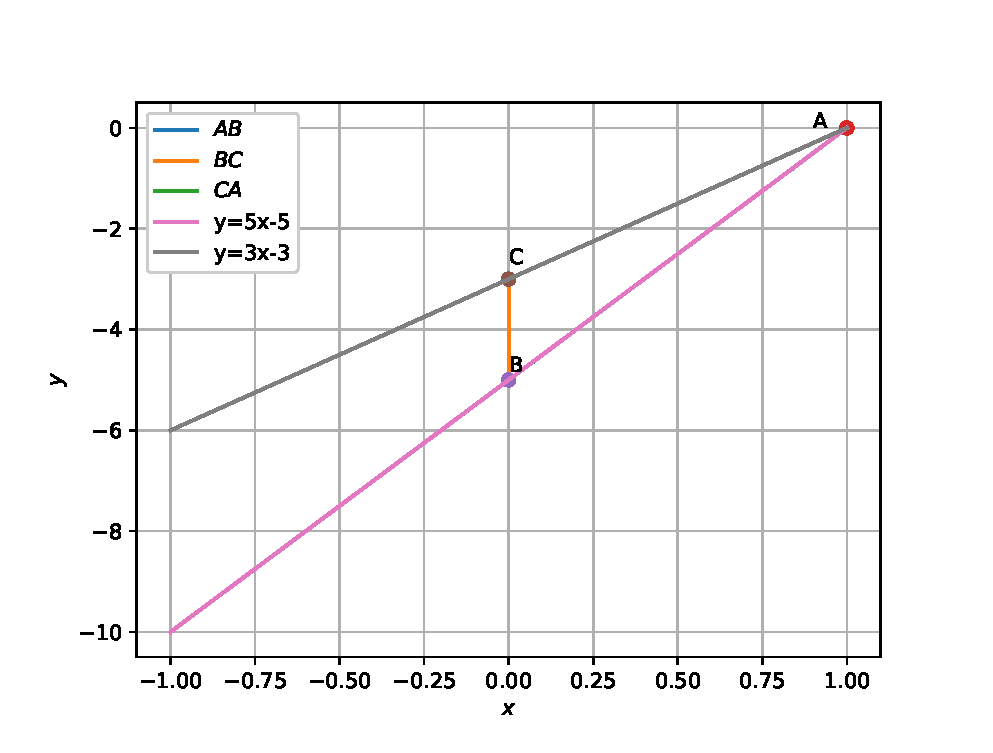
\includegraphics[width=\columnwidth]{./codes/triangle/pyfigs/triangle.eps}
\caption{Plot of lines and the Triangle ABC }
\label{fig:tri_py}
\end{figure}

\end{enumerate}
